\scanpage{75}
% Archive pencil foliation: 74.

\margin{\handwritten{On a un hom (une fois choisi $\bar{k}$ ; d'où une \unsure{réalisation|rélistion} $\deleted{\unsure{G|C|de}}'$ de lien $\underline{\unsure{\pi|\Pi}}_p(k)$) \diagram{\begin{tikzcd}\pi_1(k)\arrow[r,"K"']&G'(K)\end{tikzcd}} d'où un foncteur \diagram{\begin{tikzcd}(\text{torseurs sous }\pi_1(k)_K)\arrow[r]&\text{torseurs sous }G'\end{tikzcd}} et on prend l'image du torseur sous $\pi_1(k)_K$, défini en \unsure{interprétant|interprét} $\pi_1(k)$ comme Galois de l'extension non ramifiée \unsure{universelle|univers.|maximale} de $K$.}}
pro-fini ``abstrait'' $\handwritten{\pi}_1(k)$, mais on se convainc facilement qu'elles\deleted{et} sont contenues dans la donnée de ce groupe, $+$ son opération sur la clôture algébrique $\handwritten{\bar{K}}$ de $K$ (ou simplement, sur sa clôture non ramifiée .sur $W$ ...)\handwritten{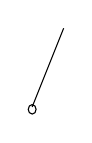
\begin{tikzpicture}[baseline=0cm,x=1cm,y=1cm]\draw[thin] (0,-.5)--(.4,.5);\draw[thin] (0,-.53) ellipse (.05 and .06);\end{tikzpicture}}. - Il resterait enfin à déterminer la structure d'effectivité dans la catégorie $\mathrm{Fcriso}(k)$ dé\unsure{\deleted{terminée}\handwritten{crite}|\deleted{terminé}\handwritten{crit}e} par la récette précédente\deleted{\unsure{.|:} la suggestion naturelle est que $\mathrm{Fcriso}^{\handwritten{+}}(k)$ est engendré par des images de $\mathrm{Fcriso}^{\handwritten{+}}$} Or il est immédiat que l'effectivité d'un F-isoc\unsure{\deleted i r|\deleted r i|\.{r}}\unsure{\deleted r i|\deleted i r|\.{r}}stal est invariante par changement de base, en particulier par le changement de base $k\handwritten{\longrightarrow\bar{k}}$, ce qui ramène au cas d'un $k$ algébriquement clos, ou encore au cas de $\underline{F}_p$ . \deleted{En}\handwritten{Dans} \deleted{termes de} la terminologie introduit e plus bas, on trouvera donc que les $\unsure{\deleted G F|\mathbb{F}|F|E}$-isocristaux effectifs sont ceux qui sont \uline{à pente} $\handwritten{\geq}0$ (i.e. dont tout es les composantes isopentiques \deleted{sont} non nulles sont de pente $\handwritten{>}\ 0$).

\handwritten{8.} Il reste donc à étudier la gerbe $\underline{G}(\underline{F}_p)$, avec s\unsure{\deleted o a|\deleted a o|a|o}\deleted{n} \deleted{foncteur fibre,} section canonique sur $\underline{Q}_p$, sa structure d'extension, et sa structure d'effectivité.

\margin{\handwritten{\figure{\begin{tikzpicture}\draw (0,0) -- (0.65,0.04) -- (0.65,0.8) -- (1.1,0.8);\end{tikzpicture}}}}
\inserted{\handwritten{8.1.}} Tout d'abord, la donnée du foncteur fibre canonique permet d'identifier $\underline{G}(\underline{F}_p)$ à la gerbe\handwritten{/}triviale définie par le lien \inserted{\handwritten{$G$}} de cette gerbe. Comme $\mathrm{Fcriso}(F_p)$ avec son foncteur fibre s'identifie à la catégorie des aut omorphismesde\inserted{$F_E$} vectoriels de dimension finie\inserted{$E$} sur $\underline{Q}_p$, avec le foncteur ``oubli de $F_E$ '', on voit que le lien de la gerbe est l'enveloppe $\underline{Q}_p$-\inserted{pro}algébriq ue d\unsure{\deleted e u|\deleted u e|\deleted a u|\deleted u a} groupe discret $\underline{Z}$ . Soit $G$ ce groupe affine sur $\underline{Q}_p$ . Il\figure{\begin{tikzpicture}[baseline=0cm,x=1cm,y=1cm]\draw[thin] (-.17,.55)--(.13,.55)--(.13,.62);\draw[thin] (-.05,.55)--(-.05,.61);\draw[thin] (-.17,-.12)..controls (.06,-.07) and (.04,-.13)..(.01,-.4);\end{tikzpicture}} est évidemment commutatif, donc produit d'un groupe vectoriel $G_u$ par un groupe de t.m. $\underset{\deleted{\unsure{G|E|m}}}{G}_r$ .
\margin{\handwritten{\unsure{réf|cf}\figure{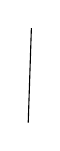
\begin{tikzpicture}\draw (0,0) -- (0.04,1.2);\end{tikzpicture}}}}
Ce dernier est l'enveloppe \inserted{de type} multiplicati\deleted{ve}\handwritten{f} du groupe $\underline{Z}$, et il s'ensuit aussitôt que c'est le groupe de t.m. dont le groupe des caractères sur $\handwritten{\bar{\underline{Q}}}_p$ est donné par
\[
\handwritten{\Gamma}=\handwritten{\bar{\underline{Q}}}_p^{\handwritten{*}}\ ,
\]
\deleted{\unsure{(|,|x}}\handwritten{(}isomorph\unsure{\deleted o i|\deleted i o}sme compatible avec l'action de $\operatorname{Gal}(\handwritten{\bar{\underline{Q}}}_p/\underline{Q}_p)$ ). D'autre
